%!TEX root = ../report.tex
\chapter{Tools and Methods}
\label{cha:background_theory}

\section{Background Theory}
The theory behind Sentiment Analysis involves a large range of concepts from both the field of machine learning and natural language processing. The natural language processing part of Sentiment Analysis is concerned with analysing and highlighting features in text, while the machine learning part is concerned with structuring and learning patterns from the features extracted.

\subsection{Support Vector Machine}
In Sentiment Analysis, machine learning has become an important and unmissable part. The most sophisticated and well performing systems today use some form of supervised machine learning where the system infers a function from labeled training data. A supervised machine learning algorithm well suited for sentiment analysis, is the Support Vector Machine. \\

The current standard incarnation of the Support Vector Machine (SVM) classification algorithm was proposed and formally described by \cite{VapnikCortes1995}. The algorithm takes a set of data points located in a feature space and attempts to split the feature space into optimal class segments. The attempt to split the feature space into optimal class segments is often referred to as \textit{training} the machine. When presented with a new unclassified data point, the data point is assigned the class of the class segment it is located in. \\

The spatial location of a data point is determined by the numerical value of its features. In a two dimensional scenario, a data point consists of two features; $x$ and $y$. If the data point is a representation of a sentence, $x$ could be the number of words in the sentence and $y$ the number of uppercase letters. In more realistic scenarios, the number of features will be much higher.  \\

In a simplified form, the algorithm solves a binary classification problem where the data is linearly separable. In that case the feature space is divided into two class segments. The class segments are separated by a hyperplane with the largest possible margin between the two segments --- this concept is called \textit{margin maximization}. The data points, closest to the hyperplane for each class, laying on a vector parallel to it, are called \textit{support vectors}. Hence the name of the algorithm: \textit{Support Vector Machine}. \\

\begin{figure}[t]
    \centering
    \begin{subfigure}[b]{0.45\textwidth}
        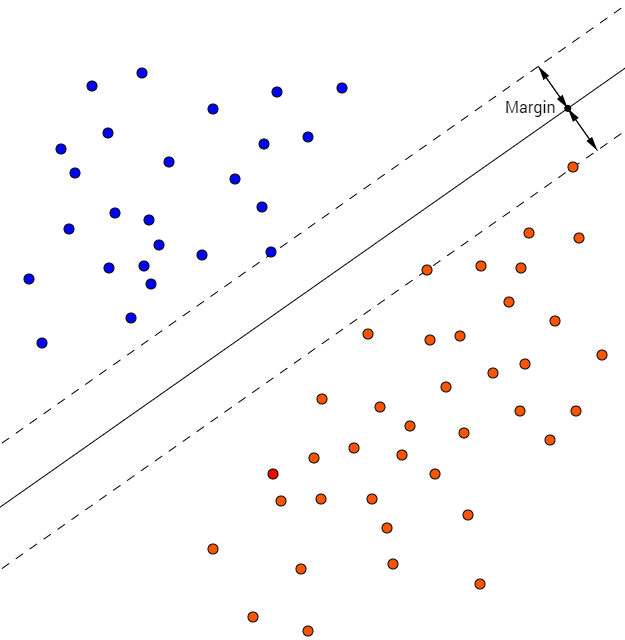
\includegraphics[width=\textwidth]{./figs/non_svm_classification_illustration}
        \caption{Non maximized margin separation}
        \label{fig:non_maximized_margin}
    \end{subfigure}
    \begin{subfigure}[b]{0.45\textwidth}
        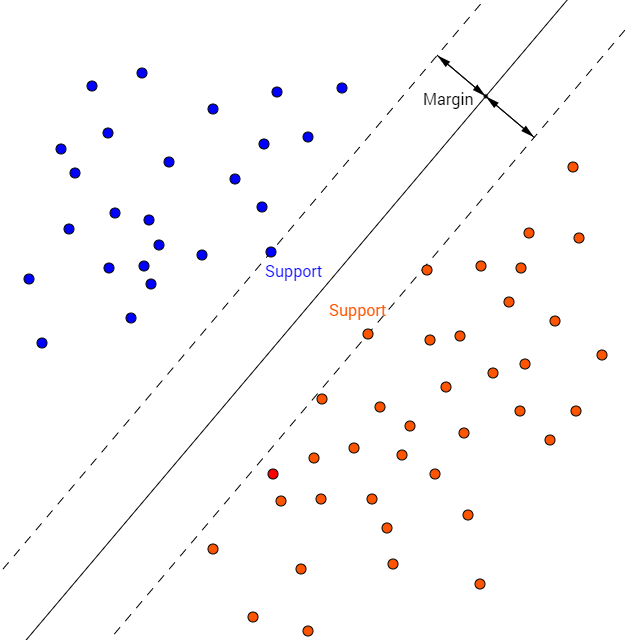
\includegraphics[width=\textwidth]{./figs/svm_classification_illustration}
        \caption{SVM maximized margin separation}
        \label{fig:svm_maximized_margin}
    \end{subfigure}
    \caption{Two possible results of linear binary classification}
    \label{fig:classification_comparison}
\end{figure}

Figure~\ref{fig:classification_comparison} illustrates two different ways of splitting the data into two classes. Figure~\ref{fig:non_maximized_margin} shows a non-maximized margin split, while Figure~\ref{fig:svm_maximized_margin} follows the SVM algorithm of finding the support vectors that result in the largest margin between the two segments. \\

The algorithm can also be used if linear separation of the training data is impossible. This could either be achieved by allowing misclassified points and introducing a slack variable, or by using the \textit{kernel trick}. In the first approach the misclassified points are assigned a penalty related to the distance away from the support vector of their class segment. The longer the distance, the higher the penalty. The penalty comes in the form of a positive slack variable, which governs the trade-off between misclassified points and the margin. \\

By using the \textit{kernel trick}, the data is mapped onto a higher dimensional space where it becomes linearly separable. This is done by applying a \textit{kernel function} to the data. The most popular kernel functions are the Radial Basis, the Polynomial and Sigmoidal kernels. The in-depth explanation of SVM by \cite{Fletcher09} states that finding the right kernel function is more of an art than an exact science. It often comes down to trial and error. \\


\begin{figure}[t]
    \centering
    \begin{subfigure}[b]{0.45\textwidth}
        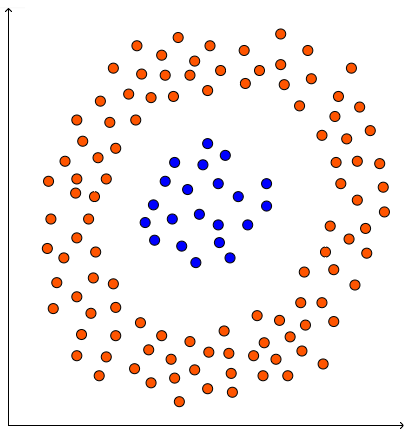
\includegraphics[width=\textwidth]{./figs/non_linearly_separable_classes}
        \caption{Before application of \textit{kernel trick}}
        \label{fig:non_linearly_separable_2d}
    \end{subfigure}
    \begin{subfigure}[b]{0.45\textwidth}
        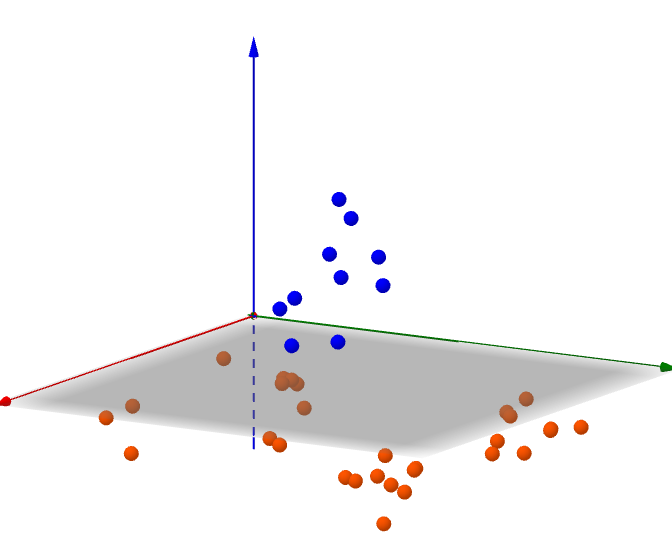
\includegraphics[width=\textwidth]{./figs/non_linearly_separable_classes_higher_dimension}
        \caption{After application of \textit{kernel trick}}
        \label{fig:non_linearly_separable_3d}
    \end{subfigure}
    \caption{\textit{Kernel trick} applied to a non-linearly separable dataset}
    \label{fig:non_linearly_separable_classes}
\end{figure}


Figure~\ref{fig:non_linearly_separable_2d} shows a dataset with a clear pattern which is not linearly separable. Figure~\ref{fig:non_linearly_separable_3d} shows the same dataset after being transformed by a kernel function to 3-dimensional space. The items occupy the same positions on the $xy$-plane, but are separable along the $z$-axis. \\

The SVM algorithm can also be applied to classification problems with more than two classes. To solve the multi-class classification problem, two methods, One-vs-All and One-vs-One, are commonly used. Both methods use a set of binary SVM classifiers and are thoroughly explained by \cite{HsuLin02}. Popular implementation of the SVM algorithm includes solving quadratic programming problems using sequential minimal optimization algorithm invented by \cite{Platt98}.


\subsection{Natural Language Processing}
\label{sec:background_nlp}
Natural Language Processing (NLP) is a branch of Artificial Intelligence concerned with processing human languages. It is a field of research within Human-Machine Interaction that aims to better the communication between humans and computers. In this project, NLP concepts such as the Bag-of-Words model and Part-of-Speech tagging have been used.

\subsection*{Bag-of-Words}
The Bag-of-Words model is a commonly used model when classifying text documents or sentences. The model, as indicated by its name, represents the text as a ``bag of words''. The \textit{bag} contains all used words and keeps track of the specific word frequencies without any structure or order. The model it creates can be used directly as a feature vector in a machine learning classifier.


\subsection*{$n$-gram}
An $n$-gram could be a single word or character appearing in a document, or a collection of words or characters appearing consecutively in a document. These two types of $n$-grams are called \textit{Word N-grams} and \textit{Character N-grams}. The $n$ in $n$-gram stands for the number of consecutive words or characters to look at.  In the \textit{Bag-of-Words} model presented above, \textit{Word N-grams} with $n = 1$ is used and the model is only looking at single independent words. With $n>1$ the same principle can be applied by treating $n$ consecutive tokens as if they were a single. 


\subsection*{Part-of-Speech Tagging}
Part-of-Speech (PoS) tagging is the process of tagging each word in a text with its lexical category. The different categories are the different parts of speech, such as: noun, verb and adjective. This categorization depends on the actual definition of the words themselves and the contexts they are in (relationships with adjacent words or other words in the text or sentence). Most PoS taggers are trained on treebanks in the newswire domain, where most of the training data is formal and well written text. The performance of these taggers commonly degrades on out-of-domain data. As stated by \cite{Gimpel11}, data such as tweets bring additional difficulties like misspellings, slang and a limited number of characters, and therefore a specialized PoS tagger for tweets is needed. 

\subsection*{Negation}
Negation in natural language is used to change the polarity of a word, a phrase or an entire sentence. Words that on their own appear to have a positive sentiment can in fact have a negative sentiment in a negated context. For example, \textit{``I am happy''} has positive sentiment, while \textit{``I am not happy''} has negative sentiment. However, negation does not always reverse the polarity entirely, sometimes negation only changes the magnitude of the polarity. For example, \textit{``I am very happy''} has high positive sentiment, while \textit{``I am not very happy''} is still positive, but not as much. \\

To negate a phrase, words called negators are used. These are also known as \textit{negation-cues} or \textit{negation-signals} and comprise words such as: \textit{not}, \textit{won't}, \textit{can't} and \textit{doesn't}. Detecting these negators in a sentence is fundamental when trying to say something about the overall sentiment of a sentence. 

\subsection*{Lexica}
Lexicon based approaches are based around the idea of calculating the overall sentiment of a text as a function of the sentiment values of the words or phrases in it. The lexica can be created manually by assigning a score to each word/phrase, or automatically. One example of automatic lexicon generation is to start with some manually classified seed words and assign a similar value to words that commonly appear together with the seed words.

\subsection*{Word Clusters}
\label{sec:background_cluster}
The word clustering technique is an attempt to reduce the data sparsity of natural languages. Instead of considering each misspelling, different grammatical forms of a word or synonyms as own and unique words, words are translated using a dictionary to a cluster ID. A common technique to generate word clusters is to use Brown clustering, by \cite{Brown92}, which is based on Hidden Markov Models. After the translation, the cluster IDs can be used in a simple Bag-of-Words model.

\subsection{Term Frequency---Inverse Document Frequency}
\label{sec:background_tfidf}
The Term Frequency---Inverse Document Frequency (TF-IDF) is a numerical statistic that provides the bag-of-words model with information about word importance. The word importance comes in the form of a weighting-scheme over all words where words with high weights provide more information than words with low weights. The actual weight each word is given is a combination of the Term Frequency ($TF$), Document Frequency ($DF$) and the Inverse Document Frequency ($IDF$) conceived by \cite{SparckJones72}. Term Frequency is the number of times a given term appears in a given document, Document Frequency is the number of documents that contain a given term, and Inverse Document Frequency is a measure of how much information a given term provides in a set of $N$ documents. The TF-IDF weight of a term within a document is calculated as follows, where $t$ is a term appearing in document $d$: \\

\begin{equation}
    \text{TF-IDF}\left(t,\, d\right) = \text{TF}\left(t,\, d\right)\cdot \text{IDF}\left(t\right)
\end{equation}

\begin{equation}
    \text{IDF}\left(t\right) = \log\frac{N}{\text{DF}\left(t\right)}
\end{equation}

As stated by \cite{Manning08}, a word will thus get a high weight if it appears often in a small amount of documents and a lower weight if it occurs few times in a document or many times across all documents. If a word occurs many times across all documents, it will get the smallest possible weight. Common words not providing much information such as: `the', `a' and `is' will therefore tend to get low weights.

\subsection{Classification Scoring Metrics}
\label{sec:classification_scoring_metrics}
To measure the performance of a classification system, a collection of scoring metrics are needed. In Sentiment Analysis the four scoring metrics: precision, recall, F1--score and accuracy are often used. The calculation of these depend on values called: \textit{true-positives}, \textit{false-positives}, \textit{true-negatives} and \textit{false-negatives}; $tp$, $fp$, $tn$ and $fn$ respectively. Here $tp$ and $tn$ are the number of examples correctly classified as positive and negative, while $fp$ and $fn$ are the number of examples falsely classified as positive and negative. This relationship can be viewed in the confusion matrix displayed in Table~\ref{tab:prediction_outcomes}.

\begin{table}[H]
    \centering
    \begin{tabular}{l|l|c|c|c}
        \multicolumn{2}{c}{}&\multicolumn{2}{c}{Predicted}&\\
        \cline{3-4}
        \multicolumn{2}{c|}{}&Positive&Negative\\
        \cline{2-4}
        \multirow{2}{*}{\rot{Correct}}& Positive & $tp$ & $fn$\\
        \cline{2-4}
        & Negative & $fp$ & $tn$\\
        \cline{2-4}
    \end{tabular}
    \caption{Confusion matrix for possible prediction outcomes.}
    \label{tab:prediction_outcomes}   
\end{table}

\subsection*{Precision}
Precision is the ratio of the number of relevant returned results to the number of total returned results. The precision ratio describes how many of the returned results are relevant. Precision is defined as:
\begin{equation*}
    precision = \frac{tp}{tp+fp}
\end{equation*}

\subsection*{Recall}
Recall is the ratio of the number of relevant results to the number of overall relevant results. The recall ratio describes how many of the relevant results are returned.  Recall is defined as:
\begin{equation*}
    recall = \frac{tp}{tp+fn}
\end{equation*}

\subsection*{$F_{1}$-Score}
F-Score is the weighted combination of precision and recall, and in its general form defined as:
\begin{equation*}
    F_{\beta} = (1+\beta)\cdot\frac{precision\cdot recall}{(\beta ^2 \cdot precision) + recall}
\end{equation*}

The most commonly used $\beta$ value is $1$, this is known as $F_{1}$-score, which produces the harmonic mean of precision and recall. $F_{1}$-score is defined as:
\begin{equation*}
    F_{1} = 2\cdot\frac{precision\cdot recall}{precision + recall} = \frac{2tp}{2tp + fp + fn}
\end{equation*}

\subsection*{Accuracy}
Accuracy is the ratio of the number of true results to the number of total cases. The accuracy ratio describes how many of the results were accurately predicted as positive and negative. Accuracy is defined as:
\begin{equation*}
    accuracy = \frac{tp+tn}{tp+fp+tn+fn}
\end{equation*}


\section{Tools}
\label{sec:background_tools}
To realize our Sentiment Analysis system, a range of programming tools where used. These tools consists for the most part of tools provided by the Python library Scikit-Learn, but in addition it also comprises a Java library for Part-of-Speech tagging created specifically for Twitter, called TwitieTagger.

\subsection{Scikit-Learn}
\label{sec:background_scikit}
Scikit-Learn, by \cite{scikit-learn}, is a machine learning library, written in Python. It consist of implementations of a wide range of state-of-the-art machine learning algorithms built for both supervised and unsupervised medium-scale problems. It emphasises ease of use and good documentation, and plays an important role in this project. In the following paragraphs the most relevant concepts and features of Scikit-Learn are presented.

\subsection*{Transformer}
A transformer object in Scikit-Learn is used to extract or generate feature representation of the data. To extract different features, different transformers must be created.

\subsection*{Pipeline}
Scikit-Learn provides a Pipeline object, allowing pipelining of machine learning processes. The pipeline makes it easy to perform and chain processes such as pre-processing and feature extraction together with a machine learning algorithm in a sequential and tidy manner. In other words, it allows sequential and parallel application of a list of estimators. An estimator is in this context either an object that is able to learn from data, such as a classifier (SVM), or a \textit{Transformer} object that extracts features from raw data. The Pipeline framework also allows performing a \textit{Grid Search} across all estimator parameters. 

\subsection*{Feature Union}
A \textit{Feature Union} is an object included in the \textit{Pipeline} framework and is a useful tool in feature extraction. The standard \textit{Pipeline} chains transformers together in a sequential manner where data from one \textit{Transformer} is fed directly into the next \textit{Transformer}. A \textit{Feature Union} on the other hand allows for a collection of transformers to be fed the exact same input data. This is especially useful when wanting to extract a series of different features from the same data. The resulting feature vectors from the transformers in the Feature Union are concatenated into a final feature matrix. 

\subsection*{Grid Search}
The \textit{Pipeline} framework allows performing a \textit{Grid Search} across all transformer or estimator parameters. The \textit{Grid Search} takes a set of possible parameter values for each parameter in each transformer and searches through all possible parameter combinations, looking for the combination that yields the best performance overall.

\subsection{Gate TwitieTagger}
The Gate TwitieTagger, by \cite{twitieTagger}, is a Part-of-Speech tagger specifically created for tweets. As described in Section~\ref{sec:background_nlp}, the Part-of-Speech tagger takes as input a sentence and returns the same sentence where each word is replaced by its part-of-speech tag. \\

Another powerful Part-of-Speech tagger tailored for tweets is the TweeboParser by \cite{Gimpel11}. TweeboParser is very complex and is written in several languages linked together with Shell and Python scripts, because of this, we decided to use the much simpler Gate TwitieTagger which is only written in Java. In terms of performance, both report a similarly high token accuracy values: 91\% and 90\% for Gate TwitieTagger and TweeboParser, respectively.

\subsection{VADER Sentiment Analysis}
\label{sec:vaderSentiment}
VADER (Valence Aware Dictionary and sEntiment Reasoner), by \cite{vaderSentiment}, is a lexicon based sentiment analysis tool specifically tuned towards social media. In contrast to our simple lexicon transformer, VADER goes beyond the simple bag-of-words model and takes into consideration word order and degree modifiers.

\section{External Data Sets}

\subsection{TweetNLP --- Twitter Word Cluster}
\label{sec:tweetnlp}
TweetNLP is a set of tools made specifically for Twitter NLP tasks. A part of TweetNLP is a hierarchical Twitter word cluster, by \cite{Owoputi12}, that was generated using Brown clustering, based on 56 million unique tweets. We have incorporated this cluster as a simple dictionary from word to cluster ID. 


\subsection{SemEval 2016 Twitter Sentiment Dataset}
As part of SemEval 2016 four data sets have been made available. These comprise a training set, a development set and a test set from SemEval 2013 and a test set from SemEval 2014. We used training and development sets for training, while the test sets was only used to test our system. To access the data sets, they all had to be downloaded through the Twitter API. Portion of the tweets have already been deleted since and are therefore no longer available. Table~\ref{tab:dataset_overview} gives an overview of the datasets used.

\noindent\begin{table}[ht]
    \begin{tabular}{| l | l | l | l | l | l |}
        \hline
         & \multicolumn{2}{c|}{\textbf{Size}} & \multicolumn{3}{c|}{\textbf{Class distribution}} \\ \hline
        \textbf{Name} & \textbf{Original} & \textbf{Downloaded} & \textbf{Positive} & \textbf{Neutral} & \textbf{Negative} \\ \hline
        2013-train & 9684 & 8748 & 3283 & 4175 & 1290 \\ \hline
        2013-test & 3813 & 3087 & 1258 & 1367 & 462 \\ \hline
        2013-dev & 1654 & 1654 & 575 & 739 & 340 \\ \hline
        2014-test & 1853 & 1509 & 794 & 564 & 151 \\ \hline
    \end{tabular}
    \caption{Overview of SemEval datasets used in the project}
    \label{tab:dataset_overview}
\end{table}

\glsresetall

